\section{Clustering Analysis}
\label{sec:clustering}

Given extracted feature data, we can model features' distributions, fit DP mixtures, fit Markov chain and eventually make implications on the results (process 2-5.1 in the modelling pipeline in \Cref{tab:pipeline}). Before that, we would like to make assumption on customer month independence and verify it through data.

\subsection{Customer Month Independence}

How does cancellation rate change over time? To see this, we group subscribers by customer month and calculate the number of each group. Suppose there are $n_t$ pupils in customer month $t$ for $t=1,\dots,T$, then the cancellation rate at $t$ is defined as $n_{t-1} / n_t$ for $t=2,\dots, T$. Recall from section \ref{sec:dataScope} that $n_1 = 2672$ and $T = 49$. We plot the evolution of number of subscribers and cancellation rate in \Cref{fig:cancellationRate}.

\begin{figure}[!h]
\centering
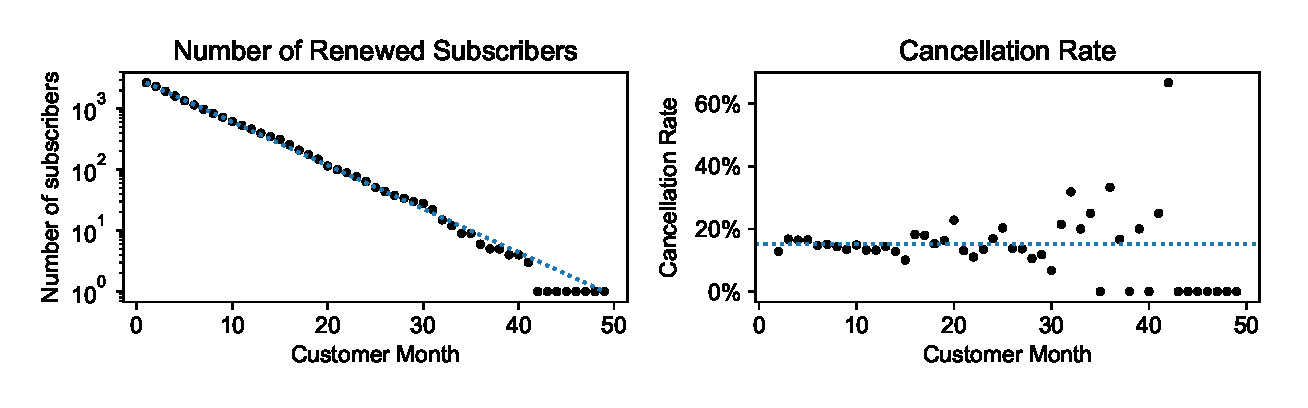
\includegraphics[scale=.7]{CancellationRate.eps}
\caption{Evolution of subscriber number and cancellation rate.}
\label{fig:cancellationRate}
\end{figure}

The vertical axis of the subscriber number plot is log-scaled. We observe that the subscriber numbers over time fit a straight dashed line very well, inferring the number is exponentially decreasing. This is again verified by a relatively constant cancellation rate over time. There comes a lot of noises when customer month is larger than 25, because after that the number of live subscribers has reduced to less than 50 so noise dominates the estimate.

Within each customer month we can assume each customer in independent from others, then we can interpret the churn rate of the customer month group as the churn probability of each individual in that group. Hence, this observation leads to a very important assumption which greatly simplifies our model: each customer's cancellation outcome is only dependent on his features within the current customer month, not further previous ones. In other words, customer months are independent in leading to churn outcome, so we can consider all customer months together and perform a single clustering. This again implies that the Markov chain is stationary, which means $A_1 = \cdots = A_T$.

As a result, in the following analysis, we will stack feature data time series $\left\lbrace \mathbf{X}_1, ~\mathbf{X}_2, ~\dots, ~\mathbf{X}_t, ~\dots, ~\mathbf{X}_T \right\rbrace$ into a single matrix $\mathbf{X} \in \mathbb{R}^{m \times n}$ with $n = \sum_{t=1}^{T} n_t$. We compute that $n=17861$.

\subsection{Distributional Modelling of Features}

We move to find appropriate density form $\phi(\cdot)$ for all $m=15$ features. We will have a visual check of their empirical distributions and also consider their correlation structure. However, we have to firstly tackle with missing data problem introduced by the way we construct features.

\subsubsection{Features with Missing Data}

It is not uncommon to observe pupils who have no visits to the service at all within a customer month although they are still in subscription. This introduces missing information to features such as mark, fail rate, etc.. We cannot simply fill these information by zeros, which are indistinguishable from real zero marks obtained by other pupils and will servrely distort the distribution if their number is large. 

We solve this problem by splitting pupils into three group partitions according to their activity level, where clustering task will be performed on different groups with different sets of features. The selection of features in each group ensure that there is no missing information or trivial information (for example, we can ignore ``number of visit'' as a feature for pupils who have no visits). We list the group definition and the associated churn rate and size in \Cref{tab:G123}. This simple splitting can already form clusters of very different churn rates. 

\begin{table}[!h]
\centering
\footnotesize
\begin{tabular}{c|p{9cm}|c}
\hline
\textbf{Group} & \textbf{Description} & \textbf{Churn rate (Size)}\\
\hline
G1 &
\textbf{Inactive:} pupils having no visits at all within the customer month. &
22.99\% (6417) \\
\hline
G2 &
\textbf{No-assess:} pupils having visits, but only take replay mode and do not take any exercise/lesson (which will give marks, pass/fail outcome) at all within the customer month. &
16.94\% (425) \\
\hline
G3 &
\textbf{Fine:} pupils having visits, and have taken exercise/lesson within the customer month. &
10.21\% (11019) \\
\hline
\end{tabular}
\caption{Group partitions of pupils due to activity level.}
\label{tab:G123}
\end{table}

\subsubsection{Independent and Multivariate Features}

The simplest form for $\phi(\cdot)$ is multivariate Gaussian where each individual feature is assumed to be a mixture of normal distributions. This appears unrealistic, even after the Box-Cox transformation. We display the empirical distributions for all features in \ref{fig:featureDistribution}. The 4 ``rate'' features at the top apparently violate the Gaussian mixture assumption. The problem comes from the phenomenon called	single-value-inflation, where a single value such as 0 has significantly frequent observations. In fact, mixture model is an ideal for modelling such distribution since it allows the overall distribution to be consisted of several different simpler distribution (not only Gaussian). We can model this feature separately from other features by assuming it is independent of other features.

\begin{figure}[!h]
\centering
\includegraphics[scale=.7, trim={0 6cm 0 0}, clip]{FeatureDistribution.eps}
\caption{Empirical distribution (histogram) and Gaussian kernel for all features.}
\label{fig:featureDistribution}
\end{figure}

Hence, we want to assume the 4 ``rate'' features to be independent from other features, and thereafter fit bespoke mixtures for each. But how likely the independence assumption holds true? We can assess the independence by at least look at the correlation structure of all features, as shown in \Cref{fig:featureCorrelation}. Incomplete rate and assess rate are very negatively correlated, but uncorrelated with other features. Fail rate and stack rate have slightly negative correlation with mark, and uncorrelated with others. Overall it seems valid to model these 4 features separately from other features, and all the other 11 features will be modelled using the multivariate Gaussian mixtures.

\begin{figure}[!h]
\centering
\includegraphics[scale=.7, trim={0 2.5cm 0 2.5cm}, clip]{FeatureCorrelation.eps}
\caption{Correlation of all features. Red stands for perfect positive correlation, blue for perfect negative correlation and white for uncorrelation.}
\label{fig:featureCorrelation}
\end{figure}




\subsection{Fitting Dirichelet Process Mixtures}

brief description of EM-algorithm and Baysian inference

\subsection{Assessing Churn Probability}

(start of the supervised learning, because of the usage of churn label)

compute cluster churn rate

interpret churn probability of individual pupil

\subsection{Feature Impact}

\subsection{Markov States Temporal Transition Analysis}

\subsubsection{Defining Markov States}

\subsubsection{Transitional Analysis}

calculate transition probability

visualise transition (matrix + Sankey plot) \cite{hmm2015}